\documentclass[conference]{IEEEtran}
\IEEEoverridecommandlockouts

\usepackage[T1]{fontenc}
\usepackage[utf8]{inputenc}
\usepackage{microtype}
\usepackage{cite}
\usepackage{amsmath,amssymb}
\usepackage{graphicx}
\usepackage{booktabs}
\usepackage{array}
\usepackage{url}
\usepackage{xcolor}
\usepackage[hidelinks]{hyperref}
\usepackage[capitalize,noabbrev]{cleveref}

\def\BibTeX{{\rm B\kern-.05em{\sc i\kern-.025em b}\kern-.08em T\kern-.1667em\lower.7ex\hbox{E}\kern-.125emX}}
\newcommand{\code}[1]{\texttt{\small #1}}
\newcommand{\RIE}{RIE}
\graphicspath{{figures/}}

\begin{document}

\title{Architecture and Empirical Characterization of a Desktop Multi-Source Scholarly Retrieval and LLM-Annotation Pipeline: The Research Intelligence Engine}

\author{\IEEEauthorblockN{Author Name(s)}
\IEEEauthorblockA{Affiliation\\
City, Country\\
email@example.org}}

\maketitle

\begin{abstract}
%%ABSTRACT%%
\end{abstract}

\begin{IEEEkeywords}
scholarly metadata aggregation, federated search, record deduplication, LLM-assisted literature analysis, Electron, fault injection
\end{IEEEkeywords}

\section{Introduction}
\label{sec:intro}

Researchers who need to survey a topic increasingly query open scholarly-metadata services directly rather than a single curated index: OpenAlex~\cite{priem2022openalex}, Semantic Scholar~\cite{lo2020s2orc,kinney2023semantic}, Crossref~\cite{hendricks2020crossref}, Europe~PMC~\cite{ferguson2021europepmc}, PubMed through the NCBI E-utilities~\cite{sayers2022eutilities}, and arXiv~\cite{arxivapi}. Coverage, metadata completeness and citation counts differ between such sources~\cite{visser2021large,gusenbauer2020which,alperin2024analysis}, so a tool that queries several of them must (i)~reconcile heterogeneous schemas, (ii)~tolerate partial failure and provider rate limits, and (iii)~remove duplicates that arise because the same work is indexed by several providers under different identifiers. Separately, large language models (LLMs) are now used to summarize individual papers, with a well-documented risk of unsupported output~\cite{ji2023survey,tang2024llmreview}.

The Research Intelligence Engine (\RIE) is an open-source desktop application (Electron~$+$ PostgreSQL) that packages these functions into one workflow: concurrent retrieval from six providers, normalization into a canonical record, in-memory deduplication, relational persistence with PDF acquisition, abstract-level LLM analysis through a hosted inference API, and a Markdown/\LaTeX{} editor. Version~1.0.0 of the code base has, to our knowledge, no published evaluation, and its README describes a narrower and partly different system than the code implements (\cref{sec:impl}).

This paper reports what can be established about \RIE{} from its source code and from controlled experiments on its actual modules. We pose four research questions.
\begin{itemize}
\item[\textbf{RQ1}] How does the implemented fan-out strategy determine end-to-end search latency and failure containment?
\item[\textbf{RQ2}] How reliably does the three-key deduplication resolve cross-provider duplicates, and which metadata disagreements defeat it?
\item[\textbf{RQ3}] What do the local components (normalization, persistence, library indexing) cost, and how do they scale?
\item[\textbf{RQ4}] How does the AI-analysis client schedule requests, recover from errors, and construct its prompt?
\end{itemize}

\textbf{Scope and honesty statement.} The sandbox in which this study was prepared blocks outbound connections to the scholarly APIs and to the LLM endpoint. We therefore \emph{did not} measure real provider latency, real retrieval effectiveness (precision/recall/nDCG), real cross-provider overlap rates, or LLM output quality, and no such number appears in this paper. Instead, the repository's real source adapters, normalizers, deduplicator, orchestrator, database layer, and AI client were executed unmodified against a deterministic \emph{emulator} of the upstream HTTP interfaces (with injected latency and faults) and a real local PostgreSQL~16 server. Everything we report as measured is a property of the \RIE{} code under those controlled conditions.

\textbf{Contributions.} (1)~A code-grounded description of \RIE's architecture, data model and pipelines, including an audit of what is implemented, validated and merely documented. (2)~A reproducible harness (fetch emulator, synthetic ground-truth corpus, fault injection, single-factor metadata perturbation) that runs the unmodified modules. (3)~Empirical findings on latency structure, failure reporting, request amplification, and deduplication behaviour, notably that the repository's deduplicator is order-dependent (non-confluent) and that its fallback key fails under every single-factor metadata disagreement we tested except letter case. (4)~A prototype relaxed-key resolver, implemented only inside the harness, whose precision/recall trade-off is quantified. \emph{Novelty statement:} the contributions are predominantly engineering and empirical; we do not propose a new algorithm, and union-find resolution and fielded matching are standard in record linkage~\cite{fellegi1969theory,elmagarmid2007duplicate,christen2012data}.

The remainder of the paper is organized as follows: \cref{sec:related} reviews related work, \cref{sec:arch} describes the system, \cref{sec:method} formalizes the pipeline and the experimental design, \cref{sec:impl} audits the implementation, \cref{sec:eval} reports experiments, and \cref{sec:disc,sec:limits,sec:concl} discuss, bound and conclude.

\section{Related Work}
\label{sec:related}

\textbf{Open scholarly metadata.} OpenAlex was introduced as an open replacement for Microsoft Academic Graph~\cite{priem2022openalex}; the Semantic Scholar corpus and data platform expose papers, citation edges and full-text-derived fields~\cite{lo2020s2orc,kinney2023semantic}; Crossref aggregates publisher-deposited DOI metadata~\cite{hendricks2020crossref}; Europe~PMC and PubMed cover the life sciences~\cite{ferguson2021europepmc,sayers2022eutilities}. Comparative studies show non-trivial differences in coverage and reference completeness among bibliographic sources~\cite{visser2021large,alperin2024analysis} and in their suitability for systematic searching~\cite{gusenbauer2020which}. Open-access PDF availability is itself uneven~\cite{piwowar2018state}, which motivates \RIE's per-provider PDF-link handling. These studies concern the sources; none evaluates a client that merges them locally.

\textbf{Federated search and tail latency.} Querying several independent engines and merging the results is the classical federated- (meta-) search problem, which involves source selection, query translation and result merging~\cite{shokouhi2011federated}; rank-fusion methods such as reciprocal rank fusion combine per-source rankings~\cite{cormack2009reciprocal}. \RIE{} performs no score fusion: it keeps the top-$k$ of each provider and re-sorts the union by year or citation count (\cref{sec:arch}). A synchronous fan-out that waits for every backend is exposed to straggler effects: the latency of the slowest component dominates, which is the central concern of ``tail-tolerant'' design~\cite{dean2013tail}. We examine that exposure for \RIE{} concretely in \cref{sec:eval}.

\textbf{Duplicate detection.} Record linkage was formalized probabilistically by Fellegi and Sunter~\cite{fellegi1969theory}; surveys and textbooks catalogue blocking keys, field-similarity metrics and clustering~\cite{elmagarmid2007duplicate,christen2012data}. Bibliographic de-duplication has been studied in the systematic-review setting, where fielded rules in reference managers and purpose-built tools differ markedly in sensitivity~\cite{bramer2016dedup,rathbone2015better}. \RIE{} uses exact-equality keys (DOI, \code{source:source\_id}, and a hash of title, first author and year). Equality keys are fast and precise but brittle under metadata variation; the experiments in \cref{sec:eval} quantify this brittleness for \RIE{} specifically.

\textbf{LLM-assisted literature analysis.} Retrieval-augmented generation grounds a generator in retrieved passages~\cite{lewis2020retrieval,gao2023retrieval}; PaperQA and PaperQA2 apply this to full-text scientific articles with evidence gathering and cited answers~\cite{lala2023paperqa,skarlinski2024language}; scite classifies the intent of citation statements~\cite{nicholson2021scite}. Unsupported generation (``hallucination'') is a documented failure mode of language generation~\cite{ji2023survey}, including fabricated references in literature-review writing~\cite{tang2024llmreview}. \RIE's analysis path is far simpler than these systems: it sends only the title and abstract plus a free-text instruction to a hosted open-weight model (default \code{openai/gpt-oss-120b}~\cite{openai2025gptoss}) and performs no retrieval, grounding or verification. We evaluate only its request scheduling and construction, not output quality.

\textbf{Positioning.} We do not benchmark \RIE{} against other tools, and we make no comparative performance claim. The paper's purpose is to characterize one system rigorously, with the harness and negative findings made available for reuse.

\section{System Architecture}
\label{sec:arch}

\subsection{Process model}
\RIE{} follows Electron's multi-process design (\cref{fig:arch}). Renderer windows (the main workbench and a separate editor window) run with \code{contextIsolation} enabled and \code{nodeIntegration} disabled; they reach the main process only through the \code{window.electronAPI} object that \code{preload.js} exposes via \code{contextBridge}, with namespaces \code{library}, \code{papers}, \code{ai}, \code{document}, \code{window} and \code{settings}. The main process (\code{electron-main.js}, plus \code{main/ipc/document-ipc.js}) registers one \code{ipcMain.handle} channel per operation and delegates to service modules. \code{paper-service.js} is the sole intermediary to ingestion, the database and the filesystem; \code{ai-service.js} wraps the hosted LLM endpoint; \code{document-service.js} spawns Pandoc for export. User-supplied API keys are persisted in a plaintext \code{settings.json} in the Electron \code{userData} directory and mirrored into \code{process.env}.

\begin{figure*}[t]
\centering
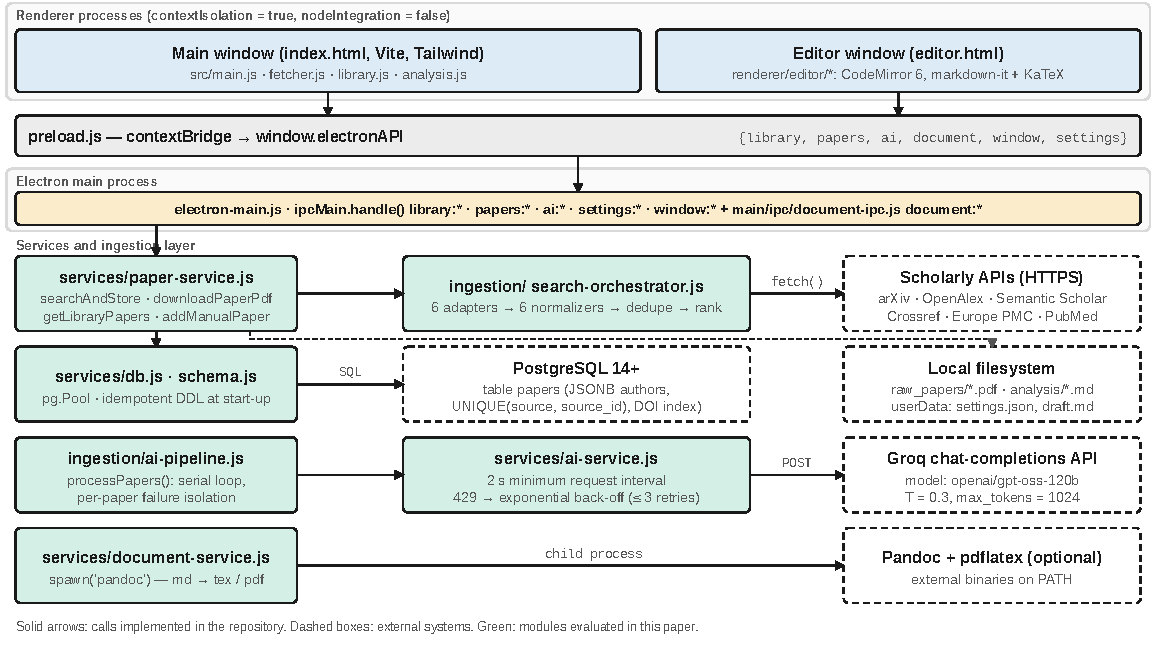
\includegraphics[width=\textwidth]{fig_architecture.pdf}
\caption{Architecture of \RIE{} as implemented in the repository (commit \code{bf2d3a3}). Renderer processes reach services only through the \code{contextBridge} API and IPC handlers. The dashed arrow from \code{paper-service.js} denotes file I/O to \code{raw\_papers/} (PDF library). Green boxes are the modules exercised by the experiments in \cref{sec:eval}; the editor and export path are described but not evaluated.}
\label{fig:arch}
\end{figure*}

\subsection{Source adapters and the canonical record}
Each provider has an \emph{adapter} (HTTP request and parsing only) and a \emph{normalizer} (mapping to a canonical record, never throwing, missing fields $\to$ \code{null}). The registry in \code{search-orchestrator.js} binds names to pairs of functions, so adding a provider requires one entry. The canonical record has twelve fields: \code{id}, \code{source}, \code{source\_id}, \code{title}, \code{abstract}, \code{authors[]}, \code{year}, \code{venue}, \code{doi}, \code{url}, \code{pdf\_url}, \code{citation\_count}. Provider-specific handling visible in the code (\cref{tab:sources}) includes reconstruction of OpenAlex abstracts from an inverted index, stripping of JATS markup from Crossref abstracts, a Crossref look-up per Europe~PMC hit to find a direct PDF link, and deliberate omission of PubMed PDF links (documented in the code as blocked by an anti-bot challenge).

\begin{table}[t]
\centering
\caption{Provider adapters as implemented (\code{ingestion/sources/*.js}). ``Req.'' is the number of upstream HTTP requests per search for limit $k$. Timeouts are the adapter's \code{AbortController} values.}
\label{tab:sources}
\footnotesize
\setlength{\tabcolsep}{3pt}
\begin{tabular}{@{}l p{0.8cm} r p{3.55cm}@{}}
\toprule
Provider & Req. & Timeout & Behaviour noted in code \\
\midrule
OpenAlex & 1 & 15\,s & $3k$ candidates, relevance sort; optional key \\
arXiv & 1 & 30\,s & $3k$ candidates; \code{ti:}\,OR\,\code{abs:}; $\geq$3\,s between calls (module-wide) \\
Semantic Scholar & 1(+1) & 15\,s & one retry after 2\,s on HTTP 429; optional key \\
Crossref & 1 & 15\,s & scholarly-type filter; \code{mailto} \\
Europe PMC & $1{+}k$ & 15\,s & per-hit Crossref look-up (3\,s timeout) for PDF link \\
PubMed & 2 & 25\,s & ESearch then EFetch (XML), 350\,ms spacing; optional key \\
\bottomrule
\end{tabular}
\end{table}

\subsection{Search pipeline}
A call \code{searchAndStore(q, sources, k, sortBy)} (\cref{fig:flow}) validates source names, dispatches all adapters concurrently with \code{Promise.allSettled}, normalizes each provider's raw items, ranks them and keeps the top $k$ per provider, deduplicates the union, assigns \code{randomUUID} identifiers \emph{after} deduplication, ranks the union again, and inserts the records into PostgreSQL. Ranking is by publication year then citation count (\code{sortBy=date}) or the reverse (\code{sortBy=citations}); records with missing values sort last. Provider relevance order is therefore \emph{not} preserved: for \code{date}, the system takes the $3k$ most relevant OpenAlex or the $3k$ most recent arXiv candidates and re-sorts them by year. The orchestrator returns the ranked list plus \code{providerStats} and \code{providerFailures} for display.

\begin{figure*}[t]
\centering
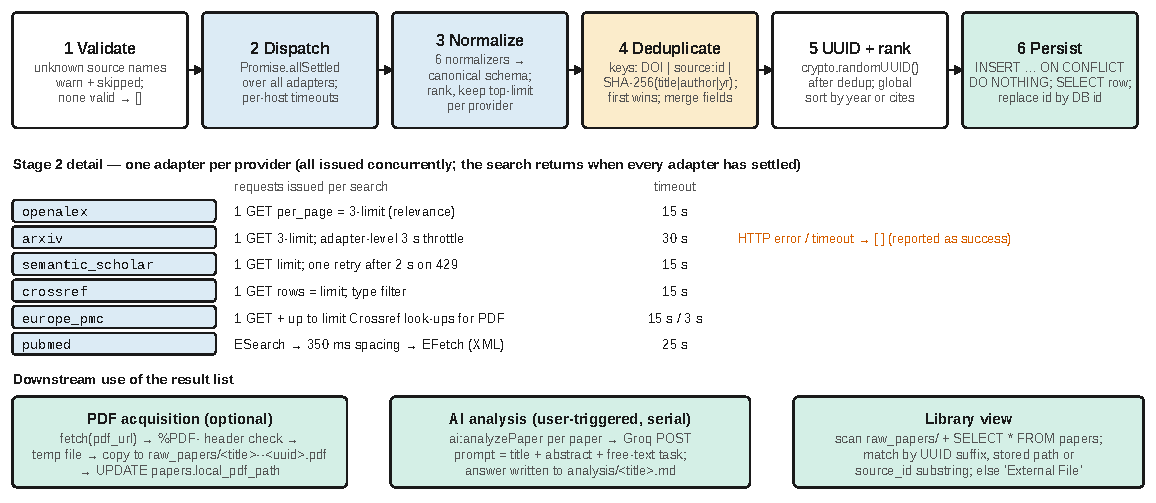
\includegraphics[width=\textwidth]{fig_dataflow.pdf}
\caption{Data flow of a search (stages~1--6), the per-provider requests of stage~2, and downstream consumers. The orange annotation marks a behaviour established in \cref{sec:eval}: an arXiv adapter failure is swallowed and appears as a successful, empty provider.}
\label{fig:flow}
\end{figure*}

\subsection{Persistence}
A single table \code{papers} stores the canonical record plus \code{created\_at} and \code{local\_pdf\_path}; \code{authors} is JSONB; \code{UNIQUE(source, source\_id)}, a unique partial index on \code{doi}, and an index on \code{created\_at} are created idempotently at start-up. Insertion is one \code{INSERT \ldots{} ON CONFLICT DO NOTHING} per record followed by a \code{SELECT} that finds the surviving row (by \code{source, source\_id} or DOI) and overwrites the in-memory \code{id} with the database identifier, so repeated searches return stable identifiers. The README additionally mentions \code{analyses} and \code{collections} tables and ``indexed full-text fields''; the schema module creates neither (\cref{sec:impl}).

\subsection{PDF acquisition, library and AI analysis}
\code{downloadPaperPdf} fetches a PDF, rejects \code{text/html} responses and bodies lacking the \code{\%PDF-} magic bytes, writes to a temporary file outside the library, copies it to \code{raw\_papers/<title>{-}{-}<uuid>.pdf}, and records a workspace-relative path. \code{getLibraryPapers} lists \code{raw\_papers/}, loads \emph{all} rows of \code{papers}, and associates files with rows by UUID suffix, stored path, or a substring test on \code{source\_id}; unmatched files are shown as ``External Document''. AI analysis is user-triggered and serial: for each paper the renderer calls \code{ai:analyzePaper}, which POSTs a chat-completion request (system prompt, then a user message containing title, abstract and a free-text task; temperature~0.3, \code{max\_tokens}~1024) to the Groq endpoint with a minimum interval between request starts (default 2\,s) and exponential back-off on HTTP~429. Each answer is written to \code{analysis/<title>.md}.

\section{Methodology}
\label{sec:method}

\subsection{Formal model of the search pipeline}
Let $\mathcal S$ be the selected providers and $T_s$ the time adapter $s$ needs to \emph{settle} (resolve or reject). Because the orchestrator awaits \code{Promise.allSettled}, the time to first result is
\begin{equation}
T_{\text{search}} = \max_{s\in\mathcal S} T_s + \varepsilon_{\text{local}},
\label{eq:tsearch}
\end{equation}
where $\varepsilon_{\text{local}}$ is the local normalize--deduplicate--rank cost. For adapters with dependent requests, and a per-request service time $L$, the code implies
\begin{align}
T_{\text{oa}} = T_{\text{s2}} = T_{\text{cr}} &= L, \quad T_{\text{ax}} = w_{\text{ax}} + L, \nonumber\\
T_{\text{epmc}} &= L + \max_{i\le k} L^{\text{cr}}_i \approx 2L, \nonumber\\
T_{\text{pm}} &= \max(L,\rho) + L, \quad \rho = 0.35\,\text{s},
\label{eq:adapters}
\end{align}
where $w_{\text{ax}}=\max(0,\,3\,\text{s}-\Delta)$ is the arXiv throttle wait given $\Delta$ seconds since the previous arXiv call started (state is module-global, so it persists across searches), and the Europe~PMC enrichment look-ups run concurrently. With a uniform $L$ this gives $T_{\text{search}} \approx \max(2L,\ \max(L,\rho)+L)$; at $L{=}0$ the PubMed spacing alone sets a floor of $\rho$. An upper bound on the worst case follows from the timeouts in \cref{tab:sources}: $T_{\text{search}} \lesssim \max(3{+}30,\ 25,\ 15{+}3,\ 2{+}2{\cdot}15)\approx 33$\,s, attained when an adapter hangs. The upstream request count for a search is $N_{\text{req}}(k) = 1{+}1{+}1{+}1{+}(1{+}n_{\text{epmc}}){+}2$ with $n_{\text{epmc}}\le k$.

\subsection{Deduplication as implemented}
For a canonical record $p$ define three keys: $\kappa_{\text{doi}}(p)$ (the lower-cased DOI without resolver prefix, if any), $\kappa_{\text{src}}(p)=(\text{source},\text{source\_id})$ (if \code{source\_id} is non-empty), and $\kappa_{h}(p)=\operatorname{SHA256}(\text{lc}(\text{title})\,|\,\text{lc}(\text{first author})\,|\,\text{year})$. Records are processed in input order; a record is a duplicate of the \emph{first} retained record that has an equal key (tested in the order DOI, source, hash), in which case missing \code{pdf\_url}, \code{abstract}, \code{venue}, \code{doi} and \code{citation\_count} of the retained record are filled from the duplicate. Otherwise the record is retained and \emph{its} keys are registered. Two properties follow directly from the code and are tested experimentally.

\emph{Property~1 (order dependence).} A duplicate's keys are not registered, even when they differ from the retained record's. Consider records $a,b,c$ of one work with $\kappa_h(a)=\kappa_h(b)\ne\kappa_h(c)$, $a$ without DOI, and $\kappa_{\text{doi}}(b)=\kappa_{\text{doi}}(c)$. For input order $(a,b,c)$: $b$ merges into $a$ via $\kappa_h$, $b$'s DOI is not registered, so $c$ matches nothing and two records are output; for order $(b,a,c)$, $a$ merges into $b$ via $\kappa_h$ and $c$ merges via the DOI, giving one record. The result thus depends on provider order and per-provider ranking, i.e., the procedure is not confluent. A transitive-closure (union-find) resolution over the same keys is order independent.

\emph{Property~2 (no negative DOI evidence).} The lookup chain evaluates $\kappa_h$ even if both records carry DOIs that differ, so differing DOIs never prevent a merge.

\emph{Cost.} Each record costs $O(1)$ hash-table operations plus one SHA-256, so the procedure is $O(n)$.

\subsection{Expected residual duplicates}
For a same-work pair in which at least one record lacks a DOI (typical for arXiv, \cref{tab:sources}) and the source identifiers differ, a merge happens only if the strict keys coincide. Writing $p_t$, $p_a$, $p_y$ for the probabilities that the normalized title, first-author string and year agree, and \emph{assuming independence}, $\Pr[\text{merge}]\approx p_tp_ap_y$ and the expected number of residual duplicates among $M$ such pairs is $M(1-p_tp_ap_y)$. We do not estimate $p_t,p_a,p_y$ for real providers; \cref{sec:eval} instead measures the response of the implementation to controlled values of each factor.

\subsection{AI-analysis scheduling}
With minimum start interval $\tau$ (default $2$\,s) and per-request latency $L_i$, the loop waits $\max(0,\tau-L_{i-1})$ after request $i{-}1$ returns, so starts are separated by $\max(L_{i-1},\tau)$ and a batch of $N$ papers takes $T_N=\sum_{i<N}\max(L_i,\tau)+L_N$ plus retries. On HTTP~429 the $a$-th retry waits $2^{a}\,\text{s}+U[0,0.5)\,\text{s}$ for $a\le m$ (default $m=3$), so $k\le m$ consecutive 429s add $\sum_{a=1}^{k}(2^a+0.25)$\,s in expectation; the $(m{+}1)$-th consecutive 429 raises the error.

\subsection{Experimental design}
\textbf{Harness.} Experiments run the repository modules unmodified under Node.js; the only substitution is \code{globalThis.fetch}, replaced by an emulator that (i)~routes by host to one of six provider mimics or the Groq endpoint, (ii)~renders records of a synthetic ground-truth corpus into the raw response shape that the corresponding normalizer reads (derived from the normalizers and the repository's own test fixtures, \emph{not} from recorded live traffic), (iii)~injects a configurable latency, and (iv)~injects faults (HTTP~500/429, network error, hang until the adapter's abort signal). Database experiments use a real PostgreSQL~16.15 server on the loopback interface with the repository's schema module. Every random choice is seeded.

\textbf{Synthetic corpus.} Works have unique titles (a numeric token guarantees no accidental collisions), 2--6 authors including names with diacritics, a DOI, a PMID, an arXiv identifier for about half the works, and a preprint year equal or one year earlier than the journal year. Because identity is known, merge outcomes are scored exactly. \emph{The corpus says nothing about real overlap rates.}

\textbf{Metrics.} \emph{Pairwise merge recall} is the fraction of same-work record pairs collapsed to one record. \emph{False merges} count distinct-work pairs collapsed. \emph{Residual duplicates} are $|\text{output}|-|\text{distinct works}|$. Timings use \code{performance.now()}; we report medians (with quartiles where $n\ge5$), discarding warm-up repetitions. Latency in the emulator is an injected parameter; measured wall-clock is compared with the models of the previous subsections.

\textbf{Platform.} 4 vCPU Intel Xeon 2.3\,GHz, 16\,GB RAM, Ubuntu 24.04, Node.js v22.23.4, PostgreSQL 16.15, single machine, no other load. \textbf{Variants.} Besides the repository's \code{deduplicate()}, two harness-only variants are evaluated: \textsc{uf-repo} (union-find over the same three keys) and \textsc{uf-relaxed} (union-find over DOI, \code{source:id}, and a relaxed key: diacritic-folded alphanumeric title, first-author surname and first initial, linked only if years differ by at most one). The relaxed key is a prototype for quantifying trade-offs, not a proposal evaluated on real data.

\section{Implementation and Repository Audit}
\label{sec:impl}

\textbf{Technology.} \RIE{} is a Node.js ES-module code base (Electron~40 shell, Vite~5 and Tailwind~3 front end, CodeMirror~6, \code{markdown-it} with KaTeX, \code{pg}~8 for PostgreSQL, \code{xml2js} for arXiv and PubMed XML). Provider calls use the platform \code{fetch} with per-adapter \code{AbortController} timeouts; the orchestrator isolates provider failures with \code{Promise.allSettled}; normalizers are total functions. \cref{tab:loc} gives size per layer (physical lines of tracked files at commit \code{bf2d3a3}, produced by \code{e0\_repo\_stats.mjs}).

\begin{table}[t]
\centering
\caption{Size of the code base by layer (physical lines).}
\label{tab:loc}
\footnotesize
\begin{tabular}{@{}l r r@{}}
\toprule
Layer & Files & Lines \\
\midrule
Ingestion: orchestration (orchestrator, dedupe, ranking, ai-pipeline) & 4 & 271 \\
Ingestion: normalizers & 6 & 720 \\
Ingestion: source adapters & 6 & 454 \\
Services (db, schema, paper, ai, document) & 5 & 746 \\
Electron main, IPC, preload & 3 & 431 \\
Renderer: main-window modules & 5 & 1\,559 \\
Renderer: editor modules & 3 & 477 \\
HTML views & 2 & 1\,057 \\
Tests & 4 & 772 \\
\midrule
Total & 38 & 6\,487 \\
\bottomrule
\end{tabular}
\end{table}

\subsection{What is implemented, validated, and documented but absent}
\cref{tab:status} separates implemented functionality from validated functionality, using (a)~the four test scripts in the repository, which we executed in the sandbox, and (b)~the experiments of this paper. Of 65 assertions executed across the four scripts, 57 passed and 8 failed; all 8 failures are live-network assertions that cannot succeed behind the sandbox's egress policy (6 in \code{test-all-providers.js}, 2 in \code{test-paper-service.js}). The 20 assertions of \code{test-workspace-library.js}, which need PostgreSQL but no network, all passed. The offline unit tests cover each normalizer with one hand-written fixture. Several assertions in \code{test-ingestion.js} are upper bounds (e.g., ``at most 6 results'') and therefore also pass when every provider returns nothing, as happened here; they do not demonstrate retrieval. There is no test of the AI service and one test of deduplication (a single pair that shares a DOI).

\begin{table*}[t]
\centering
\caption{Implementation status. ``Validated'' counts only evidence we could obtain: repository tests run here (T) or experiments in this paper (E). Live-provider and LLM-quality validation were not possible.}
\label{tab:status}
\footnotesize
\begin{tabular}{@{}p{4.2cm} p{1.6cm} p{4.3cm} p{5.7cm}@{}}
\toprule
Capability & Implemented & Validated here & Remark \\
\midrule
Concurrent retrieval from 6 providers & yes & E (emulated upstreams) & Live API behaviour untested here; repository live tests blocked \\
Normalization to canonical schema & yes & T (fixtures), E1 & One fixture per provider; no recorded live payloads \\
Deduplication (3 keys) & yes & E2 & Order-dependent; fails under single-factor metadata disagreement \\
Ranking (year / citations) & yes & E (counts only) & Relevance order discarded; retrieval quality not evaluated \\
PostgreSQL persistence, stable IDs & yes & T, E4 & Sequential per-record INSERT+SELECT \\
PDF download, library indexing & yes & T (20/20), E4 & Download path tested only by the repository suite \\
AI analysis (Groq, serial, retry) & yes & E5 (scheduling only) & Output quality, cost and rate limits not assessed \\
``Structured synthesis'', ``key contribution extraction'' (README) & partly & --- & Only a free-text prompt is sent; no output schema \\
Markdown/\LaTeX{} editor, Pandoc export & yes & --- & GUI and Pandoc not exercised \\
\texttt{analyses}, \texttt{collections} tables; full-text indexes (README) & no & --- & Schema creates only \code{papers} \\
\bottomrule
\end{tabular}
\end{table*}

\textbf{Documentation drift.} The README (i)~lists arXiv and OpenAlex as the only sources whereas six are registered, (ii)~names \code{llama-3.3-70b-versatile} whereas the code default is \code{openai/gpt-oss-120b} (git history records the change), (iii)~lists an \code{orchestrator.js} file whereas the module is \code{search-orchestrator.js}, (iv)~states that tables \code{analyses} and \code{collections} are created and that full-text fields are indexed, which \code{schema.js} does not do, and (v)~the header comment of \code{src/analysis.js} still refers to another LLM vendor. No roadmap or issue list exists in the repository, so we cannot enumerate ``planned'' work beyond the features that the README describes and the code lacks (row~10 of \cref{tab:status}).

\section{Experimental Evaluation}
\label{sec:eval}

%%EVAL%%

\section{Discussion}
\label{sec:disc}

\textbf{Answers to the research questions.} \emph{RQ1:} search latency is the maximum, not the sum, of adapter latencies, but the maximum includes adapter-internal serialization (PubMed spacing, Europe~PMC enrichment, arXiv throttle) and has no deadline, so one hung provider holds back all results until its timeout (\cref{sec:eval}); failure containment is good for five providers and misreported for arXiv. \emph{RQ2:} the deduplicator reliably merges records that share a DOI and nothing else; for DOI-less records it merges only metadata-identical strings, and the outcome depends on input order. \emph{RQ3:} local compute is negligible next to network time, but the library view re-reads and scans the whole table and scales with rows~$\times$ files in its fallback path. \emph{RQ4:} the AI client enforces a $\tau$-spaced serial schedule and bounded back-off for 429 only; it sends the literal string \code{null} for a missing abstract.

\textbf{Engineering recommendations tied to evidence.} (1)~Make adapter failure handling uniform: the arXiv adapter should reject on HTTP errors and timeouts like the other five. (2)~Add a global deadline with progressive delivery, since a single hung provider costs 15--33\,s versus sub-second typical settle times; hedged requests~\cite{dean2013tail} are inappropriate for rate-limited free APIs, so a deadline plus partial results is the proportionate response. (3)~Replace first-match deduplication by transitive closure over registered keys of \emph{all} records, which makes the output order independent, costs the same $O(n)$ (\cref{fig:scaling}), and lets a DOI veto and empty-field guards be added. (4)~Any relaxation of the fallback key (diacritic folding, punctuation-insensitive titles, surname/initial authors, $\pm1$ year) recovers the DOI-less cases but admits same-initial/same-title false merges, so it should be adopted only with a labelled evaluation on real provider data and extra evidence such as author-list overlap. (5)~Bound or defer the Europe~PMC enrichment fan-out ($k$ extra Crossref requests per search). (6)~Guard null abstracts and over-long inputs in the prompt, honour \code{Retry-After}, and retry transient 5xx responses. (7)~Batch database inserts and index the library scan if libraries grow beyond a few thousand records. These are suggestions derived from measured behaviour; we did not implement them in the application.

\textbf{Engineering contribution vs.\ scientific novelty.} The system itself is an integration of existing services and techniques; its value is practical. The scientific content of this paper is limited to (i)~an explicit, tested latency model of a federated fan-out with adapter-internal throttling, (ii)~a demonstration that a common ``first match wins'' key-based deduplicator is non-confluent and a quantification of which metadata disagreements defeat equality keys, and (iii)~a reusable fault-injection harness. None of these is a new algorithm, and none establishes retrieval or summarization quality.

\section{Limitations and Threats to Validity}
\label{sec:limits}

\textbf{No live measurements.} All upstream behaviour is emulated. Provider latency, rate-limit behaviour, error rates, payload quirks and genuine cross-provider overlap are therefore unmeasured; injected latencies are parameters, not estimates of real services, and the measured agreement with \cref{eq:tsearch,eq:adapters} shows that the code behaves as modelled, not that real searches take any particular time. The same applies to the LLM endpoint: we measured scheduling and request construction only.

\textbf{Reconstructed payloads.} Raw provider responses are rendered from the fields that the repository's normalizers read and from its own test fixtures. If real responses differ (e.g., author-name conventions, title punctuation, year semantics), residual-duplicate rates will differ. Single-factor perturbations (\cref{fig:dedup}) are deterministic properties of the key definitions and do not depend on assumed rates, but the mixed scenario of \cref{tab:e2d} depends on the assumed preprint-year skew (40\,\% of arXiv-bearing works) and abbreviated Europe~PMC author strings, and must be read as illustrative.

\textbf{Synthetic corpus and no relevance judgments.} Titles are unique by construction, which removes natural-language near-duplicates (e.g., translated titles, errata, ``Part~I/II'' series), so false-merge rates for the strict key are lower bounds on what real corpora would show and those for the relaxed key are probes, not estimates. We evaluate no query relevance, no recall against a gold standard, and no ranking quality; the year-based re-ranking may discard relevant older papers, which we neither confirm nor refute.

\textbf{Prototype variants.} \textsc{uf-repo} and \textsc{uf-relaxed} exist only in the harness; \textsc{uf-relaxed} was designed after inspecting the failure cases and tuned to nothing else, but it is untested on real data and deliberately lacks safeguards (author-list overlap, DOI veto) that a production resolver would need.

\textbf{Environment.} One machine (4 vCPU), one Node.js version, one PostgreSQL version on loopback; absolute microsecond-level timings will differ elsewhere, and PostgreSQL latency over a network would change \cref{tab:db}. The Electron GUI, the editor, Pandoc export, and the PDF download path against real publishers were not exercised; the security posture (plaintext key storage, broad IPC surface) was read from the code, not tested. Code inspection also shows that the PDF download \code{fetch} has no timeout or size limit; we did not test this.

\section{Conclusion}
\label{sec:concl}

We characterized the Research Intelligence Engine by reading its code and by running its unmodified modules against an emulated upstream environment and a real PostgreSQL server. Search latency follows the maximum of adapter latencies to within about 11\,ms in our sweep, but provider-internal throttles impose a 350\,ms floor and up to $\approx$2.6\,s of extra delay for back-to-back searches, a hung provider delays the whole result set until its timeout, and the arXiv adapter reports failures as empty successes. The deduplicator is order dependent and recovers no DOI-less duplicate under any single-factor metadata disagreement except letter case; a union-find resolver over the same keys is order independent at equal cost, and a relaxed-key prototype recovers most DOI-less cases at the price of measurable false merges. Local compute and persistence costs are small. The AI client schedules serially with a 2\,s interval and bounded exponential back-off, but silently sends \code{null} for missing abstracts. What remains open is everything that requires the live services: real latency distributions, real overlap and duplicate rates, retrieval effectiveness, and the quality of LLM analyses. The accompanying harness is intended to make such measurements easy to add once network access is available.

\section*{Reproducibility}
The complete project is in \code{paper/}: \code{main.tex}, \code{references.bib}, \code{figures/} (SVG sources, generators, PDF conversions), \code{experiments/} (harness and \code{run\_all.sh}), \code{results/} (raw JSON for every table and figure), and \code{logs/}. No application source file was modified. Experiments require Node.js~$\ge$18, \code{npm ci --omit=dev --ignore-scripts}, and a local PostgreSQL with database \code{rie\_bench} for E4; the full sweep takes roughly 20 minutes because of deliberate waits (arXiv throttle, AI interval, back-off, real timeouts). The AI experiments use a dummy API key and an emulated endpoint; no credentials were used.

\bibliographystyle{IEEEtran}
\bibliography{references}

\end{document}
